Pour pouvoir proposer de nouvelles fonctionnalités de prévention, il faut optimiser le tableau de bord et créer des logos communs à tous pour avoir le même langage. 

L'idée serait d'intégrer dans les motos une puce GPS qui serait capable d'avertir en cas de virage dangereux. L'alerte (sonore via un intercom et voyant au tableau de bord) serait envoyée via le tableau de bord connecté si la vitesse est supérieure à la vitesse recommandée. Cette vitesse sera calculée via la valeur de la courbure du virage. Des chercheurs Alex Liniger et Simon Hecker ont développé un prototype , Aegis Rider AG\cite{vitesse_virage_mcnews} permettant de prendre la meilleure trajectoire. Cependant, ce dernier ne prend pas en compte les autres facteurs de la route (autres usagers, état de la chaussée, etc.). Comme démontré ci-dessous, la trace bleu indiquant la trajectoire de sécurité et le compteur de vitesse masquent la qualité de la route par conséquent, le motard ne pourra pas anticiper les dangers de la route (gravillons, feuilles, trous et autres). À l'heure d'aujourd'hui, cette solution reste extrêmement complexe. La solution que je propose ici permettrait de fonctionner dans la plupart des cas.

\begin{figure}[H]
    \centering
    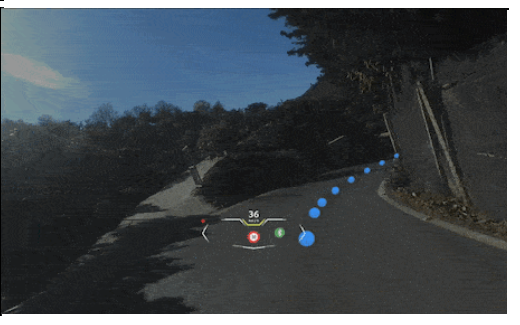
\includegraphics[width=0.7\textwidth]{coeur_memoire/images/aegis.png} 
    \caption{Prototype Aegis Rider AG pour la détection de virages dangereux.}
\end{figure}
Cette fonctionnalité est très intéressante mais elle empêche une bonne visibilité de la surface de la route et elle peut fausser une prise de décision.
Comme illustré dans la Figure~\ref{fig:trajectoire_securite_difficulte}, le processus ne pourra pas adapter sur des virages dit "imparfaits".

\subsubsection{Programme d'alerte de virages}
Le programme permet de savoir si la vitesse à l'instant T est trop rapide pour le virage. Je me base sur la valeur de la courbure.

Voici le diagramme d'action de cette fonctionnalité:\\

\begin{figure}[H]
    \centering
    \includegraphics[width=0.9\textwidth]{coeur_memoire/schéma/Capture d’écran 2025-07-24 à 17.48.10.png} 
    \caption{Diagramme d'action du Système de prévention de virages dangereux.}
\end{figure}

Pour réaliser un bout de code sur cette fonctionnalité, j'ai décidé d'utiliser ces bibliothèques :
\begin{itemize}
    \item \texttt{osmnx}\cite{osm_doc} : permet d’interroger OSM (OpenStreetMap) et de récupérer des graphes routiers.
    \item \texttt{geodesic} (de geopy \cite{geopy}) : mesure la distance réelle (en mètres) entre 2 points GPS.
\end{itemize}
\vspace{0.5cm}

Il faut convertir le graphe routier \texttt{G} (au format \texttt{NetworkX}) en un GeoDataFrame (via \texttt{GeoPandas}), pour pouvoir manipuler les tronçons de route comme des objets géographiques (segments, courbes…). Cette partie est importante pour les calculs.
\begin{lstlisting}[language=Python, caption={Conversion du graphe routier.}]
edges = ox.graph_to_gdfs(G, nodes=False)
\end{lstlisting}
Avec :
\begin{itemize}
    \item \texttt{G} : le graphe routier obtenu via \texttt{ox.graph\_from\_point} qui contient des nœuds (c'est-à-dire les intersections) et des arêtes qui représentent les routes.
    \item \texttt{nodes = False} : car je ne prends que les arêtes (edges), c’est-à-dire les segments de route. Je n'ai pas besoin pour mon programme de tous les noeuds (par exemple une intersection à plusieurs routes, un carrefour, un croisement...) du réseau. Il peut être intéressant pour calculer un plus court chemin. De plus, cela risquerait de sur-charger les données.
\end{itemize}

\vspace{0.5cm}
L'intérêt de calculer la courbure de la trajectoire est de pouvoir anticiper le virage et par conséquent, adapter la vitesse pour optimiser l'adhérence et de définir la trajectoire où l'on se sentira le plus en sécurité. \\
Le calcul de la courbure permettra d'identifier un virage s'il est dangereux à partir de données GPS cartographiques pour enfin adapter le comportement du système embarqué (alerte, adaptation de trajectoire, assistance..).
Donc la courbure mesure à quel point une route peut changer de direction sur une courte distance, ici, dans un virage.\\
Une route droite a une courbure environ égale à 0. Une route qui tourne fort (virage serré) a une courbure élevée.

\begin{table}[ht]
\centering
\begin{tabular}{|l|c|c|c|}
\hline
Route & Rayon du virage & Courbure (simplifiée) & Risque \\
\hline
Ligne droite & Infini & 0 & Faible \\
Virage large autoroute & 500 m & Faible (0.01) & Faible \\
Virage serré en montagne & 30 m & Forte (0.1–0.2) & Élevé \\
\hline
\end{tabular}
\caption{Exemple en pratique.}
\end{table}

Un virage serré avec une courbure > 0.1 est souvent dangereux à +60 km/h, surtout à moto.
Plusieurs études indiquent que les rayons < 50 m sont classés comme virages dangereux pour les motos. À plus de 60 km/h, une moto doit pencher à plus de 35°à 40° dans le virage ce qui augmente énormément le risque de chute, surtout s’il y a du gravier, pluie, vent latéral…
L’estimation “courbure > 0.1 = danger > 60 km/h” est une règle empirique, basée sur des données de sécurité moto reconnues, des normes d'ingénierie routière et des approximations géométriques issues de GPS.


L'avantage d'avoir un calcul automatique et en amont permet de prévenir avant même d'être dans le virage. Il peut remplacer un panneau quand celui-ci n'est pas visible. Elle ne remplace pas une analyse dynamique complète mais elle est suffisante pour alerter automatiquement le pilote ce qui est exactement l’objectif du système.

Je commence par créer 3 points, p1, p2 et p3, notés respectivement A, B et C sur la Figure~\ref{schemaviragepoint}, à partir des premières coordonnées GPS \texttt{position\_actuelle}. Ces trois points forment un triangle géographique.
\begin{lstlisting}[language=Python, caption={Calcul de points}]
p1, p2, p3 = coords[mid - 1], coords[mid], coords[mid + 1]
a = geodesic(p1, p2).meters
b = geodesic(p2, p3).meters
c = geodesic(p1, p3).meters
\end{lstlisting}

Pour pouvoir analyser la courbure d’un virage situé à proximité immédiate du véhicule, il est essentiel de déterminer avec précision quel segment de route (tronçon) est le plus proche (dans ce programme) de la position GPS actuelle. Pour cela, le code suivant a été utilisé :
\begin{lstlisting}[language=Python, caption={Calcul de points.}]
point_actuel = Point(position_actuelle[1], position_actuelle[0])  # (longitude, latitude)
edges["distance"] = edges.geometry.distance(point_actuel)
segment_proche = edges.loc[edges["distance"].idxmin()]
\end{lstlisting}
Pour déterminer sur quel tronçon de route se situe le véhicule, plusieurs étapes sont nécessaires.
Tout d’abord, la position GPS actuelle (latitude, longitude) est convertie en un objet géométrique de type Point, dans le format attendu par la bibliothèque shapely (longitude, latitude). Ce point matérialise la localisation du véhicule dans l’espace.
Ensuite, les segments de route issus d’OpenStreetMap (contenus dans la variable edges) sont parcourus. Chaque segment est représenté sous forme de LineString et l’on calcule sa distance par rapport au point du véhicule. Ces valeurs sont enregistrées dans une nouvelle colonne appelée distance.
Enfin, on identifie le tronçon le plus proche à l’instant T. Pour cela, on recherche simplement la distance minimale dans le tableau, puis on extrait le segment correspondant. Celui-ci représente la portion de route la plus proche de la position actuelle du véhicule.

Cette opération est cruciale car elle permet de concentrer les analyses (détection de virage, estimation de courbure, adaptation de la vitesse, etc.) sur la portion de route réellement pertinente dans le contexte de conduite.

\begin{tcolorbox}[title=Calcul de la courbure]
Courbure mathématique\cite{formule_curvature} d’un virage:
\[
courbure\_virage = \kappa = \frac{1}{R}
\]
où R est le rayon du virage\\
Forme simplifiée de la courbure basée sur la déviation par rapport à une ligne droite.\\
a, b et c sont trois points dans la courbe.\\
\[
courbure = \left| \frac{a + b - c}{a + b} \right|
\]
a + b = distance réelle parcourue en suivant la route \\
c = distance directe entre le début et la fin (comme si on traçait une corde)
\end{tcolorbox}


\begin{figure}[H]
    \centering
    \includegraphics[width=0.7\textwidth]{coeur_memoire/schéma/Capture d’écran 2025-07-22 à 16.27.35.png} 
    \caption{Schéma présentant une moto avant un virage.}
    \label{schemaviragepoint}
\end{figure}



La vitesse recommandée se calcule grâce à la courbure. Pour calculer la vitesse recommandée, conseillée, deux solutions s'offrent à moi. La première : \\
\begin{tcolorbox}[title=Vitesse recommandée]
Calcul de la vitesse recommandée :
\[
vitesse_{\text{recommandée}} = \max(20, 80-\text{curvature} \times 200)
\]
Le "20" permet d'éviter une vitesse trop basse. Ici, on la limite à 20 km/h.

\end{tcolorbox}

En dessous de 20km/h, il y a peu d'intérêt. Même les plus grosses épingles peuvent se prendre à 20km/h. À cette vitesse, il n'y a pas d'effet gyroscopique\footnote{C'est la capacité (tendance) d'un corps en rotation à maintenir une direction constante de son axe de rotation selon le Larousse.}.
Cependant, j'ai plutôt choisi de m'orienter sur des conditions simples pour catégoriser l'intensité du virage pour y associer une vitesse "maximale" qui peut être utilisée sans danger.\\
\vspace{0.5cm}
Voici comment j'ai classé la valeur de la courbure en fonction de la vitesse idéale: 
\begin{itemize}
    \item < 0.0005 → ligne droite → 80 km/h
    \item de 0.0005 à 0.002 → léger virage → 60 km/h
    \item >= 0.002 → virage serré → 30 km/h
\end{itemize}
\vspace{0.5cm}

Le fait de catégoriser la valeur de la courbure permet facilement d'y associer une vitesse. C'est une stratégie qui propose une solution plus globale en diminuant les erreurs en tests. Après avoir essayé plusieurs points GPS et analysé les virages, c'est pour moi la solution qui me convient le mieux à l'heure actuelle.
\vspace{0.5cm}


\vspace{0.5cm}
Ci-dessous le code qui permet de récupérer une localisation GPS (latitude, longitude), qui calcule la valeur de la courbure pour après estimer une vitesse de sécurité.
\lstinputlisting[language=Python, caption={Programme de calcul de la courbure et de la vitesse recommandée.}] {coeur_memoire/programme1.py}

\subsubsection{Étude de cas}
\underline{Contexte:} Lors d’une balade dans le département de Seine-et-Marne (77), un motard circule sur une route départementale. Dans ce contexte, il est équipé d’un boîtier GPS capable de récupérer ses coordonnées en temps réel, ce qui permet de suivre précisément sa position sur le réseau routier. En progressant sur son itinéraire, il arrive à proximité d’un secteur bien connu des motards locaux : la portion dite des "17 virages", située près d’Arbonne-La-Forêt.\\
Cette série de virages successifs est réputée pour sa technicité et sa dangerosité. Plusieurs facteurs viennent complexifier la conduite sur cette portion : l’état de la chaussée est dégradé, la route est étroite, véhicules arrivant en face (voitures, motos, cyclistes, bus...) et l’adhérence est souvent insuffisante, notamment en cas d’humidité ou de feuilles au sol. À cela s’ajoute un virage particulièrement critique, en forme d’équerre, qui apparaît de manière assez soudaine au milieu de la série. \\

Dans ce type de situation, adopter une trajectoire de sécurité est vivement recommandé. Le pilotage doit être précis, fluide, et adapté aux conditions réelles. Par expérience, maintenir une vitesse proche de 70 km/h, bien que ce soit la limitation autorisée, représente déjà une allure soutenue au vu de la complexité de la portion. Une bonne anticipation, une lecture fine de la route et une vitesse maîtrisée sont ici essentielles pour garantir la sécurité du motard.\\
Voici ci-dessous, une image satellite de l'endroit.

\begin{figure}[H]
    \centering
    \includegraphics[width=0.7\textwidth]{coeur_memoire/schéma/Capture d’écran 2025-07-24 à 15.45.48.png} 
    \caption{Point GPS des 17 virages.}
\end{figure}

Les coordonnées GPS sont : 48.385171, 2.563108. Afin de s'assurer de l'exactitude et du bon débogage, voici l'interprétation du réseau routier par le programme.

\begin{figure}[H]
    \centering
    \includegraphics[width=0.7\textwidth]{coeur_memoire/images/Capture d’écran 2025-07-29 à 11.39.00.png} 
    \caption{Réseau routier interprété par le programme pour la position 48.385171, 2.563108.}
\end{figure}
Voici la carte issue du traceur Géoride, attestant que l’expérience a bien été réalisée.
\begin{figure}[H]
    \centering
    \includegraphics[width=0.7\textwidth]{coeur_memoire/images/Capture d’écran 2025-07-28 à 12.07.50.png} 
    \caption{Carte du traceur Géoride arrivant sur la position 48.385171, 2.563108.}
\end{figure}
Maintenant que nous disposons du point GPS de référence, il s'agit de définir les trois points nécessaires au calcul de la courbure : p1, p2 et p3. La carte ci-dessous illustre leur positionnement précis autour du point initial.
À partir des coordonnées GPS obtenues, ici 48.385171, 2.563108 notre programme génère automatiquement les trois points suivants :
\begin{itemize}
    \item p1 : (48.3847394, 2.5636118)
    \item p2 : (48.3846809, 2.563653)
    \item p3 : ( 48.3845233, 2.56368)
\end{itemize}

\begin{figure}[H]
    \centering
    \includegraphics[width=0.6\textwidth]{coeur_memoire/schéma/Capture d’écran 2025-07-30 à 15.43.21.png} 
    \caption{Placement des points p1, p2 et p3.}
    \label{fig:cartepoints}
\end{figure}
Ces trois points, espacés dans l’environnement par rapport à la (\texttt{position\_actuelle}), permettent d’évaluer localement la courbure de ce segment routier. Cette estimation est ensuite utilisée pour calculer une vitesse de passage adaptée en accord avec les critères de sécurité fixé dans le programme.
On remarque qu'une certaine distance sépare la position actuelle (\texttt{position\_actuelle}) du point p1, ce qui permet une anticipation suffisante du virage à venir. Cette marge est essentielle pour que le motard ait le temps d'ajuster sa vitesse et sa trajectoire en fonction des caractéristiques du virage détecté.

\vspace{0.5cm}
Dans le cadre de cette mise en situation réelle, il est important de souligner que les passages étudiés ont été effectués bien avant le lancement de l’expérimentation. Ainsi, aucune donnée de vitesse n’a été relevée de manière systématique ou avec un dispositif de mesure précis à ce moment-là.\\
Chaque passage a été réalisé selon les capacités du motard au moment T, en fonction de son ressenti, de la configuration de la route et des conditions de circulation. L’objectif était avant tout d’observer un comportement naturel, sans contrainte technique imposée. Pour assurer un suivi, chaque passage a été enregistré à l’aide d’une caméra embarquée.

Voici, un premier exemple, un premier passage où la vitesse mesurée atteint 51 km/h.
\begin{figure}[H]
    \centering
    \includegraphics[width=0.6\textwidth]{coeur_memoire/images/Capture d’écran 2025-07-28 à 15.56.58.png} 
    \caption{Premier passage dans Les 17 virages aux points GPS 48.385171, 2.563108.}
\end{figure}

Résultat du premier passage avec le programme :
\begin{figure}[H]
    \centering
    \includegraphics[width=0.7\textwidth]{coeur_memoire/images/Capture d’écran 2025-07-29 à 19.53.01.png} 
    \caption{Premier passage dans Les 17 virages aux points GPS 48.385171, 2.563108.}
\end{figure}
On voit que le passage se fait à 51 km/h et que la valeur de la courbure est de 0.0006. C'est un léger virage. La vitesse estimée pour ce virage est de 60 km/h. Donc il n'y aura pas d'alerte. Voici maintenant un second passage réalisé un peu plus vite.
\begin{figure}[H]
    \centering
    \includegraphics[width=0.6\textwidth]{coeur_memoire/images/Capture d’écran 2025-07-28 à 16.35.23.png} 
    \caption{Deuxième passage dans Les 17 virages aux points GPS 48.385171, 2.563108.}
\end{figure}

\begin{figure}[H]
    \centering
    \includegraphics[width=0.7\textwidth]{coeur_memoire/images/Capture d’écran 2025-07-29 à 15.37.58.png} 
    \caption{Deuxième passage dans Les 17 virages aux points GPS  48.385171, 2.563108.}
\end{figure}

Le deuxième passage est réalisé plus rapidement (sans excès de vitesse), cependant, la vitesse est trop "rapide" pour ce virage avec une courbure de 0.0006 et il nécessite de meilleures capacités pour l'aborder. Il faut que le motard soit à un niveau intermédiaire. Comme l'objectif du programme est de faire de la prévention, j'ai décidé de me baser sur un niveau de débutant. Pour conclure, il y a un message qui apparaîtra.\\
Prenons un dernier exemple avec une nouvelle situation, une ligne droite.
\begin{figure}[H]
    \centering
    \includegraphics[width=0.7\textwidth]{coeur_memoire/images/Capture d’écran 2025-07-29 à 14.33.08.png} 
    \caption{Réseau routier interprété par le programme aux points GPS 48.514114, 2.320894.}
\end{figure}
\begin{figure}[H]
    \centering
    \includegraphics[width=0.7\textwidth]{coeur_memoire/schéma/Capture d’écran 2025-07-30 à 15.59.08.png} 
    \caption{Placement des points p1, p2 et p3 en ligne droite pour les coordonnées 48.514114, 2.320894.}
\end{figure}
Idem que pour l'exemple précédent, le programme nous génère des trois points. Avec les coordonnées 48.514114, 2.320894, voici les points que nous avons :
\begin{itemize}
    \item p1 : (48.5144999, 2.3177499)
    \item p2 : (48.5149154, 2.3148266)
    \item p3 : (48.5151433, 2.3132539)
\end{itemize}
\vspace{0.5cm}
Pour cette simulation au terminale, je décide de mettre deux vitesses, une à 80 km/h et une autre à 90 km/h. Ici je ne prends pas en compte la limitation de vitesse. Nous avons comme résultats :
\begin{figure}[H]
    \centering
    \includegraphics[width=0.6\textwidth]{coeur_memoire/images/Capture d’écran 2025-07-29 à 14.32.49.png} 
    \caption{Résultat en ligne droite pour les coordonnées 48.514114, 2.320894 à 80 km/h}
\end{figure}
\begin{figure}[H]
    \centering
    \includegraphics[width=0.6\textwidth]{coeur_memoire/images/Capture d’écran 2025-07-29 à 20.02.18.png} 
    \caption{Résultat en ligne droite pour les coordonnées 48.514114, 2.320894 à 90 km/h.}
\end{figure}
Pour conclure, comme l'usager évolue sur une ligne droite, une courbure ayant comme valeur 0 ou proche de 0, il n'y aura pas de message d'erreur qui s'affiche.

\subsubsection{Design technologique}
Afin de garantir l’efficacité du système de recommandation de vitesse sans perturber la conduite, une attention particulière doit être portée à la manière dont l’information est transmise à l’usager. Deux canaux complémentaires peuvent être mobilisés : le retour visuel et le retour sonore.\\
Pour prévenir l’usager d’un virage nécessitant une adaptation de la vitesse, il est proposé d’utiliser des pictogrammes universels, compréhensibles instantanément, sans nécessiter de lecture textuelle ou de concentration prolongée. Ces icônes pourront s’inspirer de la signalisation routière standard, par exemple un virage serré, une limitation de vitesse conseillée, une alerte "danger".
L'objectif est de minimiser le temps d’attention visuelle requis, et ainsi éviter que le motard détourne les yeux de la route.
En complément de l’affichage, un signal sonore court et identifiable peut être émis lorsque la courbure détectée dépasse un certain seuil et que la vitesse du motard est jugée excessive par rapport à la situation.
Ce bip peut remplir plusieurs fonctions :
\begin{itemize}
    \item Alerte préventive : inciter le motard à lever le pied dans un virage moyen ou serré.
    \item Alerte critique : signaler un danger si la vitesse est clairement inadaptée.
\end{itemize}
Pour ne pas créer de gêne ou de stress, le signal doit :
\begin{itemize}
    \item Être court, non strident et facilement reconnaissable,
    \item Être désactivable ou réglable par l’utilisateur (volume, type de son),
    \item Ne pas se répéter en boucle inutilement, afin de respecter l’attention du motard.
\end{itemize}
L’ajout de ce canal auditif permet d’éviter la dépendance au visuel et s’adresse particulièrement aux utilisateurs préférant rester concentrés sur la route sans consulter un écran.
Le système devra permettre une personnalisation des retours utilisateur, afin de s’adapter aux préférences et aux besoins de chacun :
\begin{itemize}
    \item Possibilité d’activer ou désactiver le son,
    \item Choix du mode d’alerte (visuel seul, sonore seul, ou les deux),
    \item Réglage de la sensibilité des alertes (par exemple, activer uniquement pour les virages très serrés).
\end{itemize}
Cela garantit une expérience utilisateur plus inclusive, tenant compte des profils variés : motards expérimentés, jeunes conducteurs, ou encore personnes malentendantes.

\begin{figure}[H]
    \centering
    \includegraphics[width=0.4\textwidth]{coeur_memoire/images/Capture d’écran 2025-07-25 à 14.42.42.png} 
    \caption{Génération d'un tableau de bord possible avec l'IA.}
\end{figure}

Il pourrait être intéressant de poursuivre le développement sur une action sur les freins afin de ralentir légèrement la moto ou bien empêcher ou couper l'accélération. C'est une piste intéressant  mais cependant, il faut prendre en considération plusieurs facteurs : 
\begin{itemize}
    \item Ne pas surprendre le motard,
    \item Ne pas diminuer l'adhérence des pneus,
    \item Ne pas influencer sur la trajectoire de sécurité, or la vitesse joue un rôle crucial dans la trajectoire.
\end{itemize}
